
\documentclass[10pt]{beamer}

\usepackage{media9}
\usepackage{amssymb,amsmath,amsthm,enumerate}
\usepackage[utf8]{inputenc}
\usepackage{array}
\usepackage[parfill]{parskip}
\usepackage{graphicx}
\usepackage{caption}
\usepackage{subcaption}
\usepackage{bm}
\usepackage{amsfonts,amscd}
\usepackage[]{units}
\usepackage{listings}
\usepackage{multicol}
\usepackage{multirow}
\usepackage{tcolorbox}
\usepackage{physics}
\usepackage[english]{babel}
\usepackage{fancyvrb}
\usepackage{xcolor}
\usepackage{listings}
\usepackage{wrapfig}

% Enable colored hyperlinks
\hypersetup{colorlinks=true}

% The following three lines are for crossmarks & checkmarks
\usepackage{pifont}% http://ctan.org/pkg/pifont
\newcommand{\cmark}{\ding{51}}%
\newcommand{\xmark}{\ding{55}}%

% Numbered captions of tables, pictures, etc.
\setbeamertemplate{caption}[numbered]

%\usepackage[superscript,biblabel]{cite}
\usepackage{algorithm2e}
\renewcommand{\thealgocf}{}

% Bibliography settings
\usepackage[style=ieee]{biblatex}
\setbeamertemplate{bibliography item}{\insertbiblabel}
\addbibresource{references.bib}


\theoremstyle{remark}
\newtheorem*{remark}{Remark}
\theoremstyle{definition}

\newcommand{\empy}[1]{{\color{darkorange}\emph{#1}}}
\newcommand{\empr}[1]{{\color{cardinalred}\emph{#1}}}
\newcommand{\examplebox}[2]{
\begin{tcolorbox}[colframe=darkcardinal,colback=boxgray,title=#1]

\end{tcolorbox}}

\usetheme{Madrid} 

\title[Air Quality Forecasting]{Air Quality Forecasting}
\addtobeamertemplate{footline}{\hypersetup{allcolors=.}}{}
\begin{document}

\author[]{Datena Maria Alfredo, Dell'Atti Martina, Palummo Alessandro}
\date{November 20, 2020}

\begin{frame}\maketitle
\begin{figure}[h]
    \centering
    
\includegraphics[width=0.2\linewidth]{polimi.jpg}
\end{figure}
\end{frame}


\setbeamertemplate{itemize items}[default]
\setbeamertemplate{itemize subitem}[circle]


\begin{frame}{Wiseair}

     Wiseair is a startup born in 2018 from some students of Politecnico di Milano, who focused on the problem of \textbf{air quality}.
     \\They designed low-cost sensor called \textbf{Arianna}, which
measure the concentration of Particulate Matter once per hour
    \begin{figure}[h]
	\centering
	
\includegraphics[width=0.6\linewidth]{wiseairArrapato.jpg}
\end{figure}
\end{frame}

\begin{frame}{Dataset}
    Wiseair own 68 air quality sensor in Milan at the moment, active from July 2020, and they are increasing day by day thanks to the involvement of citizens who installed them. 
    Our data go from September 2020 to November 2020
    \begin{figure}[h]
	\centering
	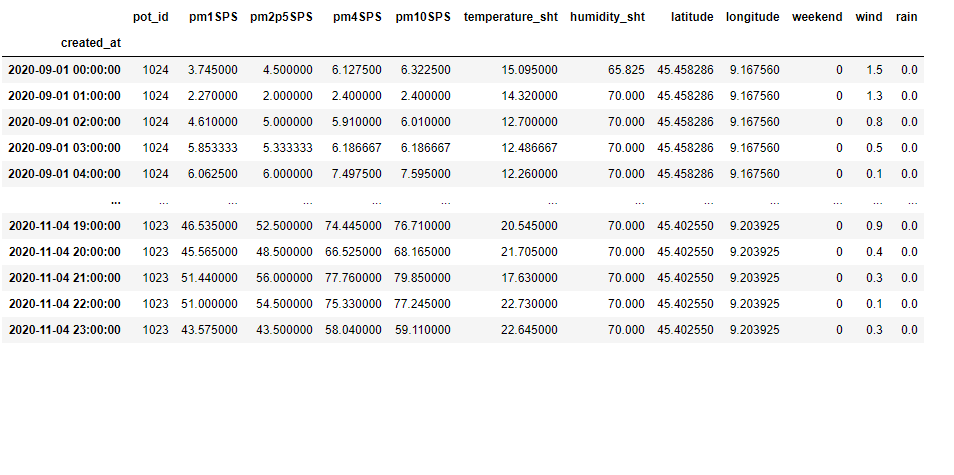
\includegraphics[width=1\linewidth]{dataset.png}
\end{figure}
\end{frame}

\begin{frame}{Dataset}
\begin{itemize}
    \item < 1->  \textbf{pot-id} identifies which sensor has taken the measurement. The ID is useful to geolocate the measurement
    \item < 2 -> \textbf{created-at} gives the time coordinate for the measurement, up to the second. The format is "yyyy-mm-dd hh:MM:ss"
    \item < 3 -> \textbf{pm1SPS}, \textbf{pm2p5SPS}, \textbf{pm10SPS} are the Particular Matter, pollutant of the air, which have dimensions, respectively, less or equal than $1 \mu m$, $2.5 \mu m$, $ 10 \mu m$. 
    They are measured in $\mu g/m^{3}$
    \item < 4 -> \textbf{temperature-sht, humidity-sht} are the temperature and the humidity for each sensor's measurement of Arianna
    \item < 5 -> \textbf{latitude, longitude} 
    \item < 6 -> \textbf{weekend} is a dummy variable which indicate if the measurement is in a day of the week or not \item < 7 -> \textbf{wind, rain} are the wind speed and the rain level measured by ARPA sensors 
\end{itemize}
\end{frame}

\begin{frame}{Data Exploration}
    \begin{figure}
        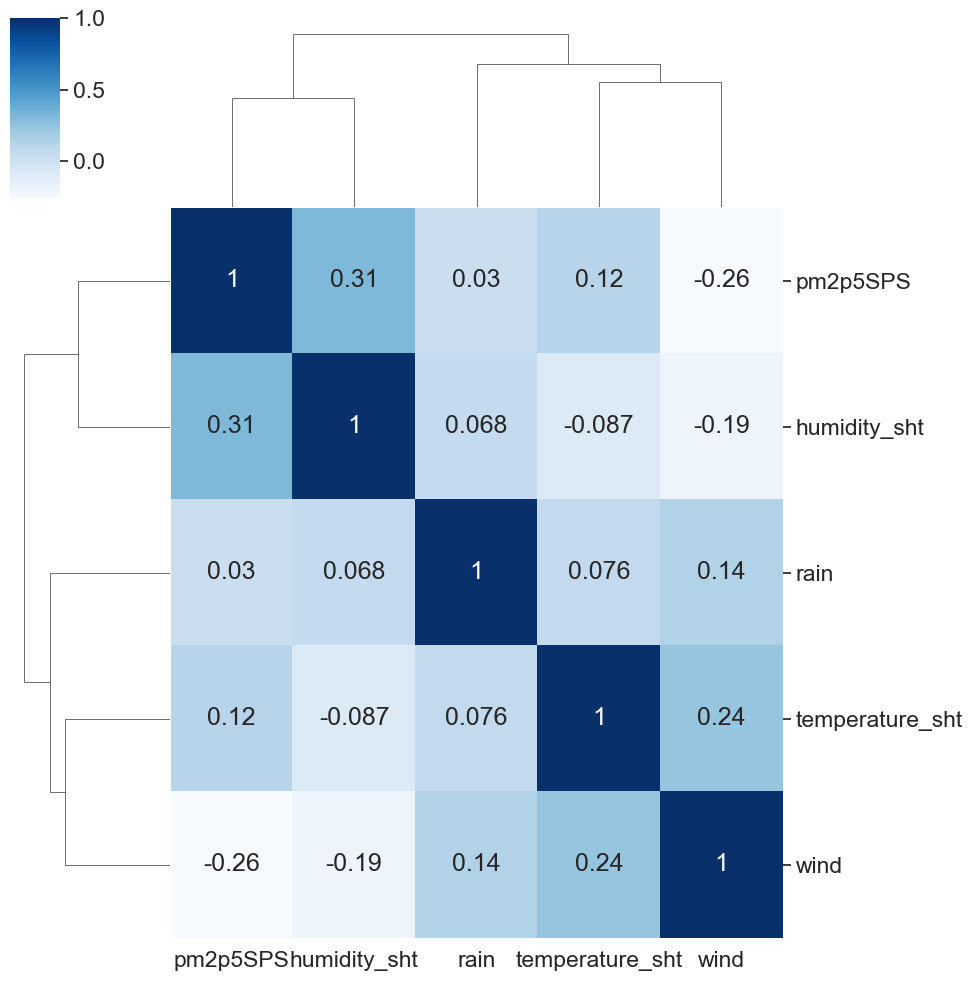
\includegraphics[scale=0.2]{correlation.png}
    \end{figure}
 From domain knowledge we know that sensors tends to measure higher PM values if humidity increases a lot. The clustermap, which plot a matrix dataset as a hierarchically-clustered heatmap, put in evidence the correlation between humidity and pm2p5 values, which is higher w.r.t. the correlation between the other features. 
\end{frame}
\begin{frame}{Goal}
Our main \textbf{goal} is to predict future PM values. \\
We will tackle the problem in two steps:
    \begin{itemize}
        \item \textbf{Univariate analysis}: focus on a single time series without taking into account any spatial correlation between different sensors.
        \item \textbf{Multivariate analysis}: derive a vectorial model which uses information from all the sensors, this time taking into account the spatial correlation between them.
    \end{itemize}
    \begin{figure}[h]
        \centering
        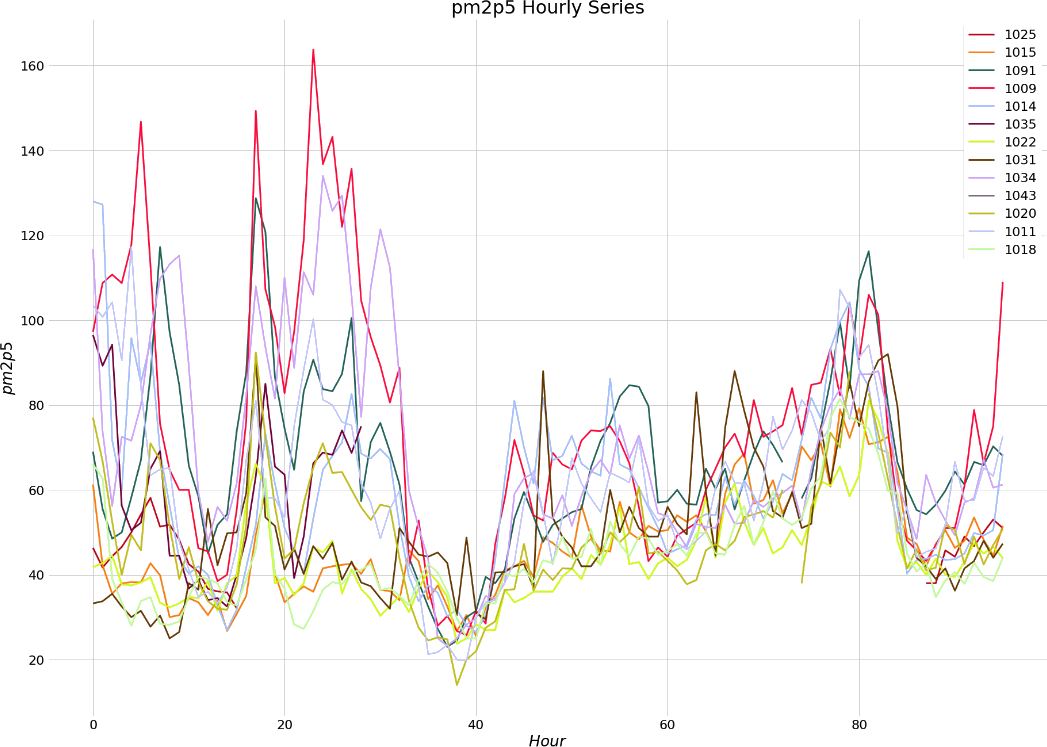
\includegraphics[scale=0.15]{plotDati.png}
    \end{figure}
\end{frame}


\begin{frame}{The model}
    The first proposed model for Univariate Analysis is an AR(2) model:
\begin{equation*}
    y_t = \phi_1 y_{t-1} + \phi_2 y_{t-2} + \epsilon_{t} \qquad \qquad \epsilon_{t} \sim \mathcal{N}(0, \sigma^2) 
\end{equation*}
where $\epsilon_{t}$ is a sequence of uncorrelated error terms and the $\phi_i$ are constant parameters.

\vspace{3mm}
\begin{columns}
\column{0.3\textwidth}
        \text{LIKELIHOOD}\newline\newline
        \begin{aligned} 
        y|\underline{\phi},\beta & \sim \mathcal{N}(\underline{\phi}^{T}\beta,\sigma^{2})\\
        & \text{$\sigma^{2}$ not known}
        \end{aligned}
\column{0.4\textwidth}
        \text{PRIORS}\newline\newline
        \begin{aligned}
	    \underline{\phi }|\sigma^2 &\sim \mathcal{N}_2(\underline\mu_0, \sigma^2B_0) \\
        \sigma^2 &\sim inv\Gamma \Bigl(\frac{\nu_0}{2}, \frac{\nu_0 \sigma_0^2}{2} \Bigr) \qquad \\
        &\text{ $\mu_0, B_0, \nu_0, \sigma_0^2$ fixed}
        \end{aligned} 
\end{columns}
\end{frame}

\begin{frame}{Why AR(2)?}
    \begin{figure}[h!]
        \centering
        \begin{minipage}[t]{0.4\textwidth}
          \centering
          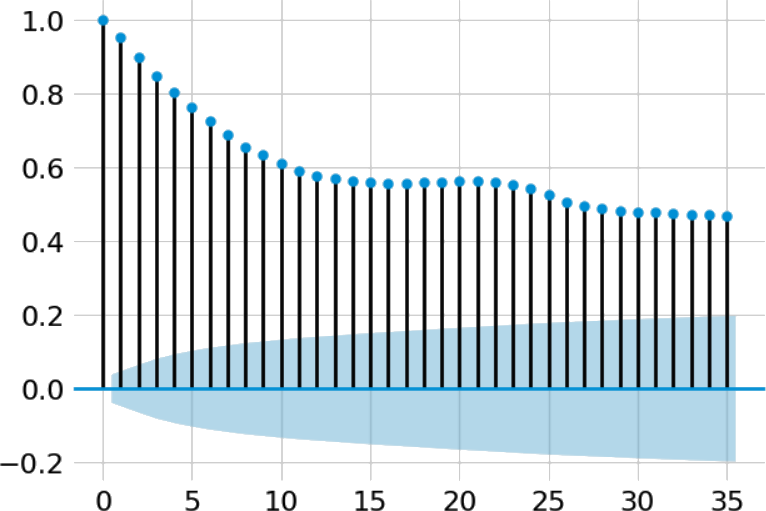
\includegraphics[scale=0.2]{acf.png}
        \end{minipage}\hfill
        \begin{minipage}[t]{0.6\textwidth}
          \centering
          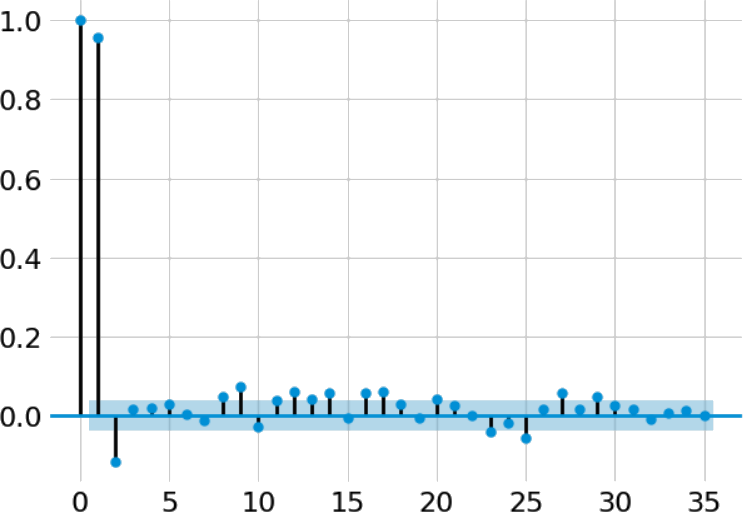
\includegraphics[scale=0.2]{pacf.png}
        \end{minipage}
    \end{figure}
    ACF tends to zero only asymptotically, while PACF drops to zero at lag 2. An autoregressive model of order 2 seems the most appropriate choice.
\end{frame}

\begin{frame}{The model}
Since the model is a standard conjugate linear model,\\
the  POSTERIORS are:

\begin{center}
      \begin{itemize} 
  \item $\underline{\phi }|Y \sim \mathcal{N}_2 (\mu_n, \sigma^2 B_n)$
  \end{itemize}
  \end{center}
  \begin{align*}
      \mu_n &= \mu_0 + B_0 \Phi[\Phi^{T} B_0 \Phi + I_n]^{-1}(Y - \Phi^T\mu_0) \\
      B_n &= B_0 - B_0\Phi[\Phi^{T} B_0 \Phi + I_n]^{-1}\Phi^T B_0
  \end{align*}
       
\begin{center}
\begin{itemize}
\item   $\sigma^2 | Y &\sim inv\Gamma \Biggl(\frac{v_n}{2}, \frac{v_n \sigma_n^2}{2} \Biggr)$ 
\end{itemize}
\end{center}
\begin{align*}
    v_n &= v_0 + n \\
    \sigma_n^2 &= \frac{1}{v_n} \Bigl[ v_0\sigma_0^2 + (Y - \Phi^T\mu_0)^T [\Phi^T B_0 \Phi + I_n]^{-1} (Y - \Phi^T\mu_0) \Bigr]
\end{align*}
            
\end{frame}

\begin{frame}{Future model development}
    We do not expect that a simple AR(p) model will work. This is just a first attempt to understand the structure of the time series. Next steps:
    \begin{itemize}
        \item try to fit more "complex" classical TS models as ARMA/ARIMA
        \item include seasonality in the model by fitting a SARIMA model (we have spotted a daily seasonal component)
        \item pass to a Dynamic Linear Model formulation (poi spiego meglio...) 
        \item extend the scalar case to the vectorial case, introducing spatial correlation between different sensors
    \end{itemize}
\end{frame}
\begin{frame}{Bibliography}
\begin{itemize}
    \item Time Series Modeling, Computation,and Inference. 
\vspace{3mm}
West Mike, Prado Raquel
\item Quadro di riferimento ambientale, Componente Atmosfera - Istituto superiore per la protezione e la ricerca ambientale(ISPRA) 

\end{itemize}
    
\end{frame}

\end{document}